\documentclass{beamer}
\usepackage{sdp}

\title{Файлове}

\titlegraphic{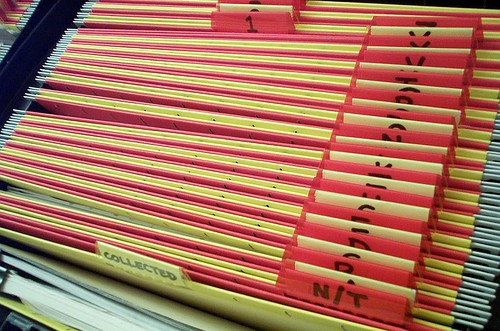
\includegraphics[width=0.5\textwidth]{images/files.jpg}}

\begin{document}

\begin{frame}
  \titlepage
\end{frame}

\begin{frame}
  \frametitle{Какво е файл?}

  \begin{itemize}
  \item Блок информация, записана на траен носител
  \item Разлика между масив и файл
  \item Файлови системи
  \item Метаданни на файла
  \end{itemize}
\end{frame}

\begin{frame}
  \frametitle{Файлът като поток}
  
  \begin{itemize}
  \item Последователен достъп
  \item Еднопосочно обхождане
  \item Еднократна обработка
  \item Краен поток
  \item Файлът може да играе ролята на
    \begin{itemize}
    \item производител (входни файлове)
    \item консуматор (изходни файлове)
    \end{itemize}
  \end{itemize}
\end{frame}

\begin{frame}
  \frametitle{Файлът не е само поток}

  \begin{itemize}
  \item Пряк достъп
  \item Разширяване при запис
  \item Едновременно четене и запис
  \end{itemize}
\end{frame}

\begin{frame}
  \frametitle{Текстови файлове}
  \begin{itemize}
  \item Форматиран вход и изход
  \item Само последователен достъп
  \item Еднократно обхождане
  \item Интерпретиране на данните във файла като текст (ASCII, Unicode или др.)
  \item Прилича на низ
  \end{itemize}
\end{frame}

\begin{frame}
  \frametitle{Двоични файлове}
  \begin{itemize}
  \item Неформатиран (суров) вход и изход
  \item Позволява пряк достъп
  \item Многократно обхождане
  \item Интерпретацията на данните във файла зависи от конкретната задача
    \begin{itemize}
    \item  масив от числа
    \item структура
    \item масив от структури
    \end{itemize}
  \end{itemize}
\end{frame}


\begin{frame}
  \frametitle{Поточна йерархия в C++}

  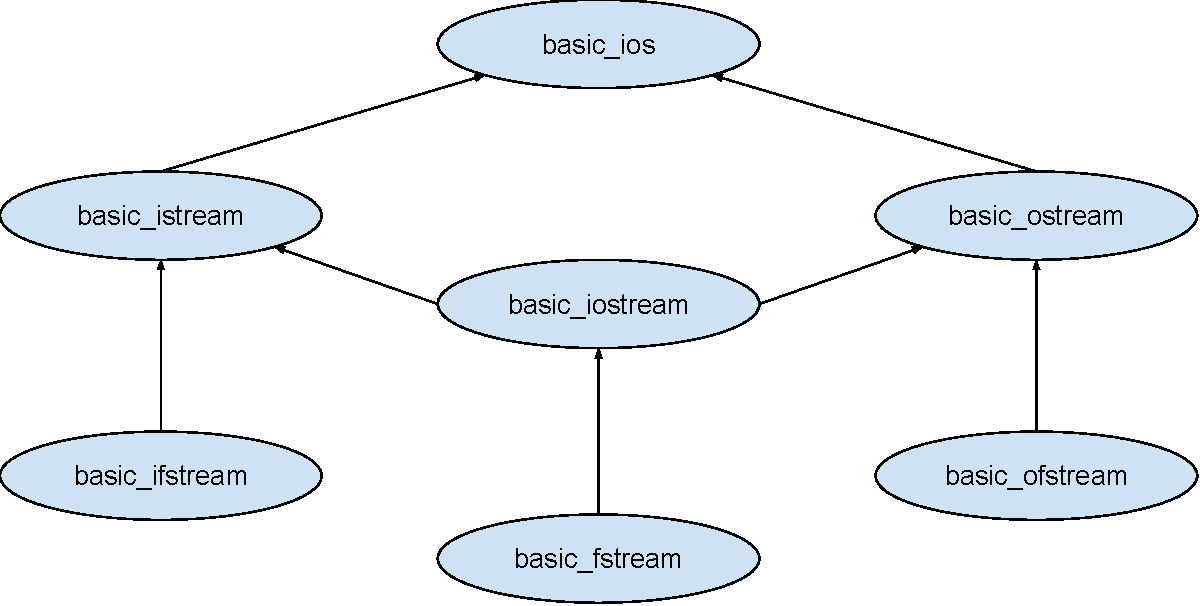
\includegraphics[width=\textwidth]{images/stream_hierarchy.pdf}
\end{frame}

\begin{frame}[fragile]
  \frametitle{Входни файлове}

  \verb#ifstream(char const*, openmode = ios::in )#
  \vspace{1em}

  \begin{itemize}
  \item \verb#void open(char const*, openmode = ios::in)#
  \item \verb#void close()#
  \item \tt{ios::binary} — суров (неформатиран) вход
  \end{itemize}
  \vspace{3em}

  Примери:
\begin{verbatim}
ifstream fi("email.txt", ios::in );
ifstream fi("lolcat.jpg", ios::in | ios::binary );
\end{verbatim}
\end{frame}

\begin{frame}[fragile]
  \frametitle{Изходни файлове}

  \verb#ofstream(char const*, openmode = ios::out|ios::trunc)#
  \vspace{1em}

  \begin{itemize}
  \item \verb#void open(char const*, openmode)#
  \item \verb#void close()#
  \item \tt{ios::trunc} --- отрязва (унищожава) файла
  \item \tt{ios::ate} --- вмъкването става в края
  \item \tt{ios::app} --- вмъкването винаги е в края
  \end{itemize}
  \vspace{1em}

  Примери:
\begin{verbatim}
ofstream fo("page.html", ios::out );
ofstream fo("application.log", ios::out | ios::app );
ofstream fo("file.dat", ios::out | ios::binary );
\end{verbatim}

\end{frame}

\begin{frame}[fragile]
  \frametitle{Входно-изходни файлове}

  \verb#fstream(char const*, openmode = ios::in | ios::out)#
  \vspace{1em}
  
  Пример:
\begin{verbatim}
fstream f( "essay.txt" );
f.getline(line, 100);
f << "Ignore the following text, please!";
\end{verbatim}
\end{frame}

\begin{frame}[fragile]
  \frametitle{Пряк достъп до файлове}

  Отправна точка за преместване на текущата позиция:

  \begin{tabular}{|c||c|c|c|}
    \hline
    seekdir&beg&cur&end\\
    \hline
  \end{tabular}
  \vspace{2em}

  Селектори:
\begin{verbatim}
streampos tellg() const
streampos tellp() const
\end{verbatim}

  Мутатори:
\begin{verbatim}
istream& seekg(streampos, seekdir = beg)
ostream& seekp(streampos, seekdir = beg)
\end{verbatim}

\end{frame}

\begin{frame}[fragile]
  \frametitle{Структурирани файлове}

  \begin{center}
    \newcommand{\yc}{\cellcolor{yellow}\hskip 1ex}
    \newcommand{\gc}{\cellcolor{green}\hskip 1ex}
    \newcommand{\bl}{\multicolumn{4}{c}{$\underbrace{\hskip 7ex}_{\tt{Student}}$}}
    \begin{tabular}{|c|c|c|c|c|c|c|c|c|c|c|c|c|c|c|c|c|c|c|c|c|c|c|c|}
      \hline
      \yc&\yc&\yc&\yc&\gc&\gc&\gc&\gc&\yc&\yc&\yc&\yc&\gc&\gc&\gc&\gc&\yc&\yc&\yc&\yc&\gc&\gc&\gc&\gc\\
      \hline
      \bl&\bl&\bl&\bl&\bl&\bl
    \end{tabular}
  \end{center}
  \vspace{1em}

\begin{verbatim}
class Student { ... };

Student s;
f.seekp( i * sizeof (Student) );
f.write((char const*)&s, sizeof(Student));

Student sa[3];
f.seekg( j * sizeof(Student) );
f.read( (char*)sa, 3 * sizeof(Student));
\end{verbatim}
\end{frame}

\begin{frame}
  \frametitle{Задача ``СУСИ''}

  \begin{itemize}
  \item Да се въведе списък от студенти
  \item Да се запише в текстов файл \tt{students.txt}
  \item От \tt{students.txt} да се прочетат студентите, които не са скъсани и да се запишат в главната книга \tt{main.bk}
  \item В главната книга да се повиши с 1.0 оценката на студент с даден Ф№
  \end{itemize}
\end{frame}

\end{document}
